\section{Anforderungsanalyse}
Das folgende Kapitel analysiert den bestehenden Prozess zur Ressourcenübersicht
beim \gls{HOD} Systemtest. Basierend auf dieser Analyse wird der Soll-Zustand 
des Projekt definiert, indem genaue Anforderungen an das System gestellt werden. 
Diese Anforderungen werden priorisiert, um anschließend die Funktion des 
fertigen Systems zu validieren.

\subsection{Analyse des aktuellen Testprozesses}
Aufgrund der Mitgliedschaft von mehreren Jahren bei \gls{JSS} und der Entwicklung
von mehreren Programmen, die diesen Prozess automatisieren oder unterstützen, Infrastruktur
mir der Prozess äußerst bekannt. Dennoch wurden Interviews mit den Hauptbeauftragten
der unten beschriebenen Rollen durchgeführt. Um den Prozess besser zu verstehen,
wurden UML Aktivitätsdiagramme erstellt. Da die Rollen teilweise wenig 
miteinander interagieren, wurden die Prozesse der jeweiligen Rollen einzelnen
betrachtet.\\

Der aktuelle Testprozess basiert auf einem täglich erstelltem Tagesplan 
(Siehe~\ref{fig:tagesplan}). Dieser Tagesplan beinhaltet die Tests, welche an diesem
Tag von den \gls{Techniker}n durchgeführt werden sollen, mit den wichtigsten 
Informationen, wie zum Beispiel das Programm zur Reihenfolge der simulierten Griffe.
Da diese Liste als Jira Auszug in Form einer \gls{PDF} oder statische \gls{HTML} Datei zur Verfügung 
gestellt wird, kann sie keinerlei Informationen zu vorherigen oder folgenden 
Tests liefern, welche jedoch für einen effizienten Umbau benötigt werden.

Weiterhin gibt es keinerlei Informationen zu Wartungszeiten der einzelnen Ressourcen.
Diese müssen in einer separaten Ressourcenliste eingesehen werden
(Siehe~\ref{fig:ressourcenliste}). Die Aktualisierung dieser Liste findet nur über 
das Versionskontrollsystem \gls{SVN} statt und liegt verborgen in einer Vielzahl
an Ordnern. Zusätzlich muss der Start der Benutzung der Ressource eingetragen
werden. Dadurch muss die Liste nach einer Wartung erneut angepasst werden. So 
ergeben sich die folgenden Prozesse:

\begin{figure}[H]
    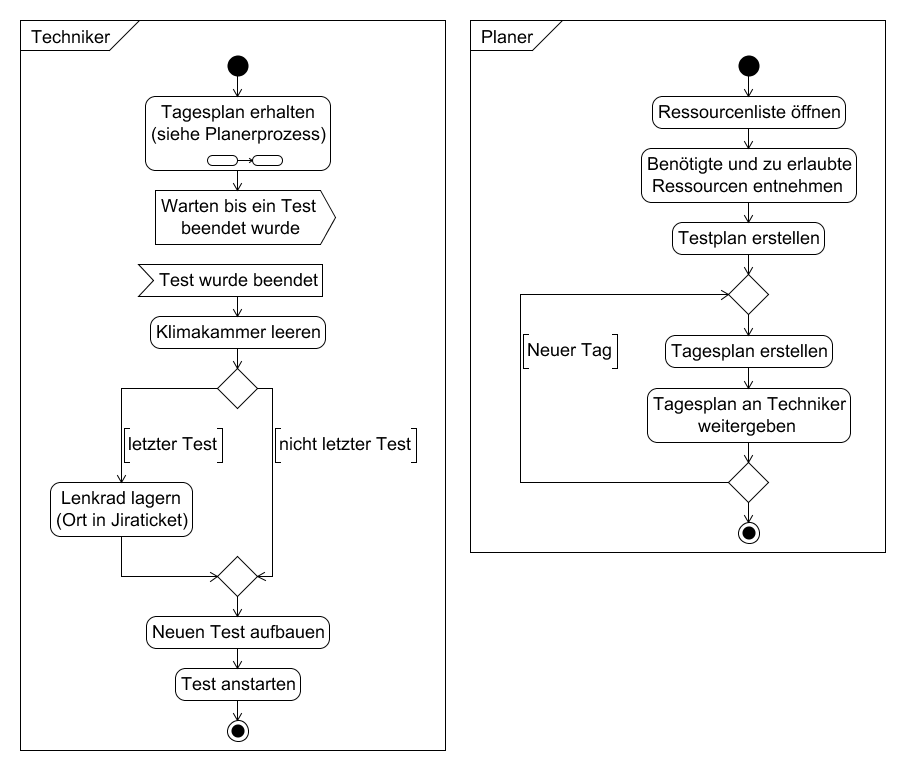
\includegraphics[width=\linewidth]{diagramme/TechnikerPlanerProzess.png}
    \caption{UML Aktivitätsdiagramm zum täglichen Testprozess}\label{fig:TechnikerPlanerProzess}
\end{figure}

Aus Abbildung~\ref{fig:TechnikerPlanerProzess} gehen zwei verschiedene Rollen hervor. Der
Planer (rechts) ist verantwortlich für das langfristige Planen von Tests. Dabei muss
dieser beachten, dass die Wartungstermine eingehalten werden, wenn
eine gewisse Ressource eingeplant wird. Welche Ressourcen überhaupt zur
Verfügung stehen und wann die Wartungstermine überhaupt sind, kann der Planer aus
der Ressourcenliste entnehmen. Zusätzlich erstellt der Planer auch den täglichen 
Tagesplan, welcher nur das Ergebnis eines \gls{JQL} Filters ist. 

Der Techniker (links) hingegen, ist für den Umbau und die tatsächliche Durchführung der 
Tests verantwortlich. Er benötigt den Tagesplan um zu wissen, welche Tests als 
nächstes durchgeführt werden. Da im Tagesplan allerdings nicht vermerkt ist, 
welcher Test nach eine spezifischen Test durchgeführt werden muss, muss er die 
Klimakammer so weit es nötig ist leeren, um anschließend den nächsten Test 
aufzubauen. Zusätzlich weiß er nicht, welcher Test der letzte einer Testgruppe ist.
Diese Information ist nötig, um die anschließende Lagerung des Lenkrads einzuleiten.
Um diese Information zu erhalten, muss er im jeweiligen Jira Ticket nachschauen. \\

\begin{figure}[H]
    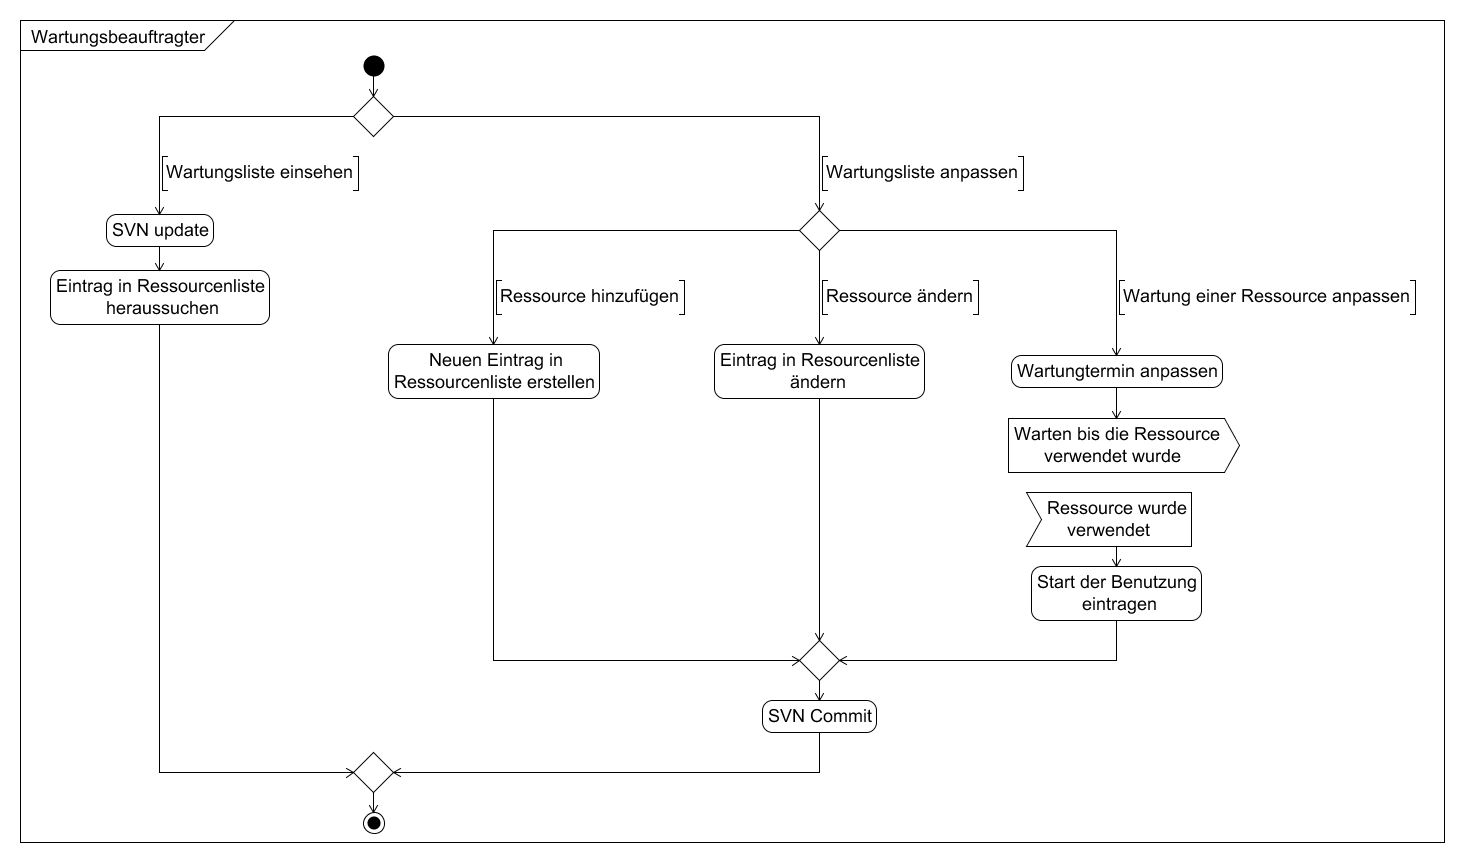
\includegraphics[width=\linewidth]{diagramme/WartungsbeauftragterProzess.png}
    \caption{UML Aktivitätsdiagramm zum Ressourcenmanagementprozess des Wartungsbeauftragten}\label{fig:WarterProzess}
\end{figure}

Der in Abbildung~\ref{fig:WarterProzess} beschriebene Prozess zeigt den Umgang mit der 
Ressourcenliste. Der Wartungsbeauftragte muss jedes mal, wenn er die Wartungsliste
einsehen will, vorher ein \gls{SVN} Update machen, um auch tatsächlich die aktuelle
Version der Liste zu erhalten. Wird dies nicht getan, kann es bei Änderungen 
zu \gls{SVN} Konflikten kommen oder die entnommenen Informationen sind veraltet.
Falls er irgendetwas an der Liste anpasst, muss diese anschließend wieder ins 
\gls{SVN} hochgeladen werden, um die Informationen mit allen anderen Mitarbeitern
zu synchronisieren. Zusätzlich muss zu jedem neuen Wartungstermin, das tatsächliche
Datum der ersten Benutzung seit der Wartung eingetragen werden.

Somit ergeben sich die folgenden Rollen:

\begin{description}
    \item[\textbf{Planer}] Die Rolle der Person, die Pläne für kurzfristige oder
    langfristige Tests erstellt.

    \item[\textbf{Wartungsbeauftragter}] Die Rolle der Person, die Wartungen 
    überwacht, plant und durchführt. 

    \item[\textbf{Techniker}] Die Rolle der Person, die Tests aufbaut, umbaut und
    durchführt
\end{description}

Auch wenn es sein kann, dass eine Person mehrere Rollen annimmt, ist es dennoch 
wichtig die Rollen voneinander zu unterscheiden um den Prozess nachvollziehbarer
und übersichtlicher zu gestalten.

\subsection{Einbindung in vorhandene Programme}
Da gerade die Wartungsinformationen auch in anderen Programmen benötigt werden, 
beispielsweise um Warnungen bei abgelaufener Wartungen bei der Testvorbereitung
anzeigen lassen zu können, ergibt sich eine weitere Rolle:

\begin{description}
    \item[\textbf{Entwickler}] Die Rolle der Person, die die Informationen der
    offenen Schnittstelle für eigene Programme verwendet
\end{description}

\subsection{Use Cases}
In Abbildung~\ref{fig:usecases} und Abbildung~\ref{fig:usecasesEntwickler} sind 
die bereits definierten Rollen als Akteure dargestellt.
Die Use Cases ergeben sich aus den Interviews.

\begin{figure}[H]
    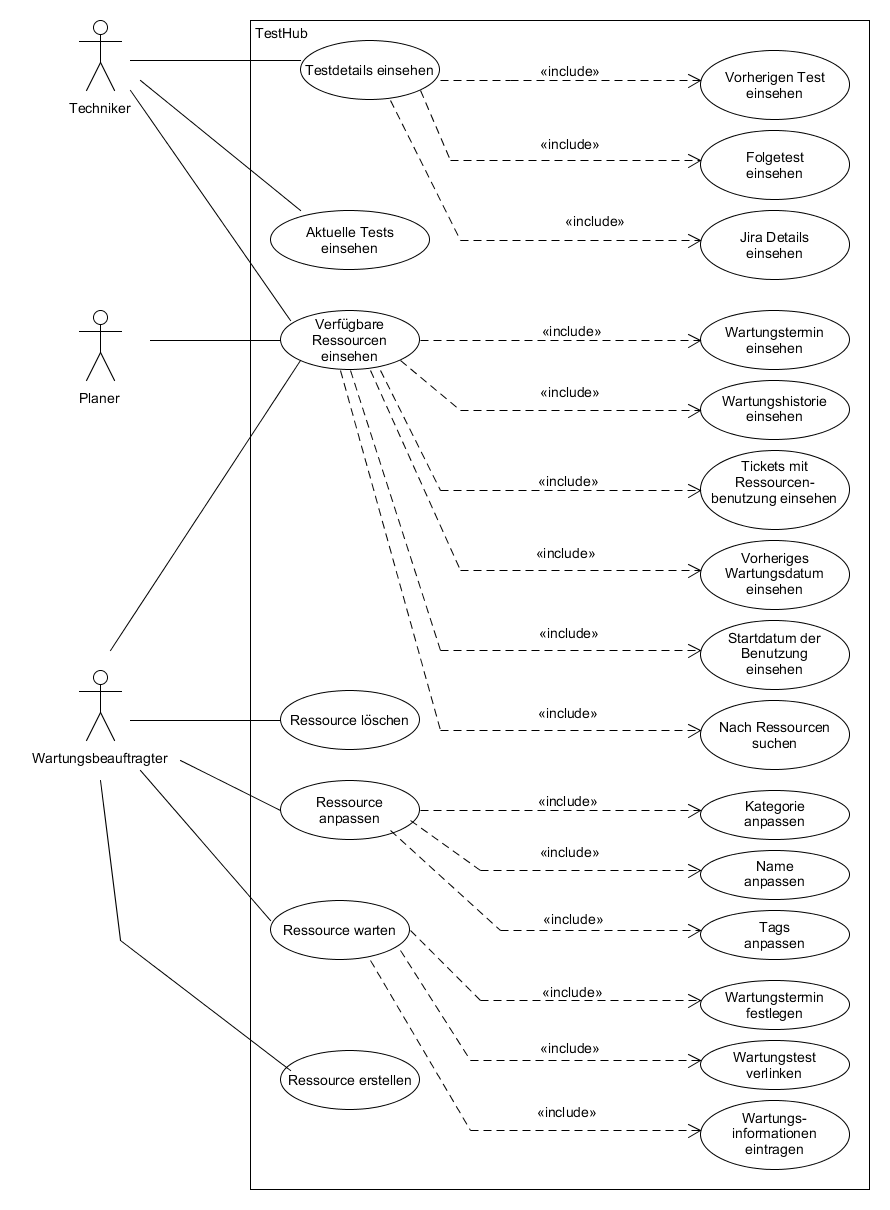
\includegraphics[width=\linewidth]{diagramme/Usecases.png}
    \caption{UML-Use-Case-Diagramm zu den Anwendungsfällen für die Planer-, Techniker- und Wartungsbeauftragten-Rolle}\label{fig:usecases}
\end{figure}

\begin{figure}[H]
    \includegraphics[width=\linewidth]{diagramme/UsecasesEntwickler.png}
    \caption{UML-Use-Case-Diagramm zu den Anwendungsfällen für die Entwickler-Rolle}\label{fig:usecasesEntwickler}
\end{figure}

\subsection{User Stories}
Die User Stories ergeben sich aus den Use Cases.

\begin{description}
    \item[\textbf{US\#01}]\textit{Als Techniker möchte ich einen vorherigen Test
    einsehen}

    \item[\textbf{US\#02}]\textit{Als Techniker möchte ich einen folgenden Test
    einsehen}

    \item[\textbf{US\#03}]\textit{Als Techniker möchte ich die Details eines Jiratickets
    in aufgeschlüsselter Form einsehen}

    \item[\textbf{US\#04}]\textit{Als Techniker möchte ich alle aktiven Tests einsehen}

    \item[\textbf{US\#10}]\textit{Als Planer möchte ich einen Wartungstermin einsehen, um zu erfahren
    ob ich diese Ressource einplanen kann}

    \item[\textbf{US\#11}]\textit{Als Planer möchte ich eine Wartungshistorie einsehen, um eventuelle
    vergangene Probleme aufzudecken}

    \item[\textbf{US\#12}]\textit{Als Planer möchte ich alle aktiven Tickets sehen, 
    welche eine spezifische Ressource verwenden}

    \item[\textbf{US\#13}]\textit{Als Planer möchte ich das vorherige Wartungsdatum einsehen, 
    um zu wissen, ob das Startdatum der Benutzung hinter dem Wartungsdatum liegt
    und ich somit die Ressource verwenden kann}

    \item[\textbf{US\#14}]\textit{Als Planer möchte ich das Startdatum der Benutzung einsehen,
    um zu wissen, ob das Startdatum der Benutzung hinter dem Wartungsdatum liegt
    und ich somit die Ressource verwenden kann }

    \item[\textbf{US\#15}]\textit{Als Planer möchte ich nach Ressourcen suchen}

    \item[\textbf{US\#20}]\textit{Als Wartungsbeauftragter möchte ich eine Ressource löschen}

    \item[\textbf{US\#21}]\textit{Als Wartungsbeauftragter möchte ich die Kategorie 
    einer Ressource anpassen}

    \item[\textbf{US\#22}]\textit{Als Wartungsbeauftragter möchte ich den Namen 
    einer Ressource anpassen}

    \item[\textbf{US\#23}]\textit{Als Wartungsbeauftragter möchte ich die Tags 
    einer Ressource anpassen}

    \item[\textbf{US\#24}]\textit{Als Wartungsbeauftragter möchte ich einen neuen 
    Wartungstermin festlegen}

    \item[\textbf{US\#25}]\textit{Als Wartungsbeauftragter möchte ich das Ergebnis eines
    Wartungstest verlinken}

    \item[\textbf{US\#26}]\textit{Als Wartungsbeauftragter möchte ich Informationen
    zu einer Wartung speichern}

    \item[\textbf{US\#27}]\textit{Als Wartungsbeauftragter möchte ich eine Ressource erstellen}

    \item[\textbf{US\#90}]\textit{Als Entwickler möchte ich die REST API verwenden, um die
    Informationen von ``TestHub'' in meine Programm einzubinden}

    \item[\textbf{US\#91}]\textit{Als Entwickler möchte ich die Dokumentation
    der API ansehen, um zu verstehen wie ich die API benutzen kann}

\end{description}

\subsection{Funktionale Anforderungen}